% !TeX root = ../thuthesis-example.tex

\chapter{THE VR-IOT RESEARCH PLATFORM}

Before the platform's development, several meetings were held to discuss key implementation details and the architecture of the VR-IoT research platform, or, as it was named later, "NUIX-Studio."

Based on the first meeting discussion, it was decided that the main functionality of the platform would be:
\begin{enumerate}
     \item Visualization of devices;
     \item Interaction with devices;
     \item Simulation of device sensors.
\end{enumerate}

The NUIX-Studio API must provide an API for different interaction techniques and simulation of device sensors inside virtual reality.

After several brainstorming sessions, it was proposed to divide device controls into touch interface interaction and other interaction methods, such as voice control, sight control, gesture control, etc. The ability to control devices at a distance impossible to perform in real life, such as lengthening the arms, dropping hands, etc., was allocated to a separate category. These control methods could be used in the real world in the future by introducing new technologies such as holographic projection.

To preserve the narrative structure, the author introduces only the final platform prototype in this chapter.

\section{Platform requirements}
Based on the literature review, the platform should follow these minimum requirements:
\begin{enumerate}
\item Scalability. The performance of the platform should stay acceptable when the number of devices in the system increases. Otherwise, the latency of the synchronization between the devices inside VR-IoT environment will increase to a level when the system is unable to perform Data analysis for the research;
\item Ease of use and testing. Users need to efficiently use the NUIX-Studio API and platform tools to create new IoT devices and test them in the VR-IoT environment.
\item Fault Tolerance. The platform should effectively handle faults coming from both real and virtual worlds to provide a valuable user experience;
\item Simultaneous work. As in the real world, where several people can interact with an IoT system at the same time, each of the platform's running instances should be able to run simultaneously and operate with the same data.
\end{enumerate}

By dividing the NUIX-Studio structure into these three layers, the platform becomes more resilient (Figure~\ref{fig:BasicPlatformStructure-figure}): 
\begin{enumerate}
    \item Real-world IoT devices HUB is a special device responsible for receiving and sending data to real-world devices that provides the data in a unified format (abstraction of sensors) for the middle layer. An open-source software openHAB (\cite{OpenHab}) is used with a future upgrade to a standalone solution to support different IoT devices. The HUB runs on a server and is responsible for storing the IoT devices' data. Managing the data is performed through a Web Interface;
    \item Integration layer is responsible for analyzing data coming from VR and real-world, integrating real-world devices data into VR and vice-versa, performing persistence, and providing API for using the platform in research projects. By receiving and sending unified data objects representing IoT devices' sensor data using REST API calls, each of the NUIX-Studio App instances operates with the same data, enabling simultaneous work. The next step is to represent IoT devices' data in Virtual reality and perform computations for research. Since the platform should run smoothly on VR headsets and provide good UX, the analysis should be performed on a powerful PC\footnote{In Chapter 4 an experiment proving this statement is provided.}. At the same time, Virtual reality headsets perform computations for interacting with objects, such as hand recognition;
    \item Visualization layer. Interaction with digital IoT devices can be performed using VR headsets, AR devices, or simulating touch, sight, gestures, and other interactions. The platform provides an API for developers to integrate their interaction techniques into this layer, but developing these techniques is not the focus of this research. It was decided to use Unity (\cite{Unity}) for interaction with virtual reality devices. Firstly, Unity comes with a ready-to-use 3D engine, relieving the need to develop a new one. Secondly, Unity is multi-platform and supports VR headsets. Thirdly, developers are already familiar with Unity development, making it easier for them to integrate the platform into their solutions.
\end{enumerate}

\begin{figure}
  \centering
  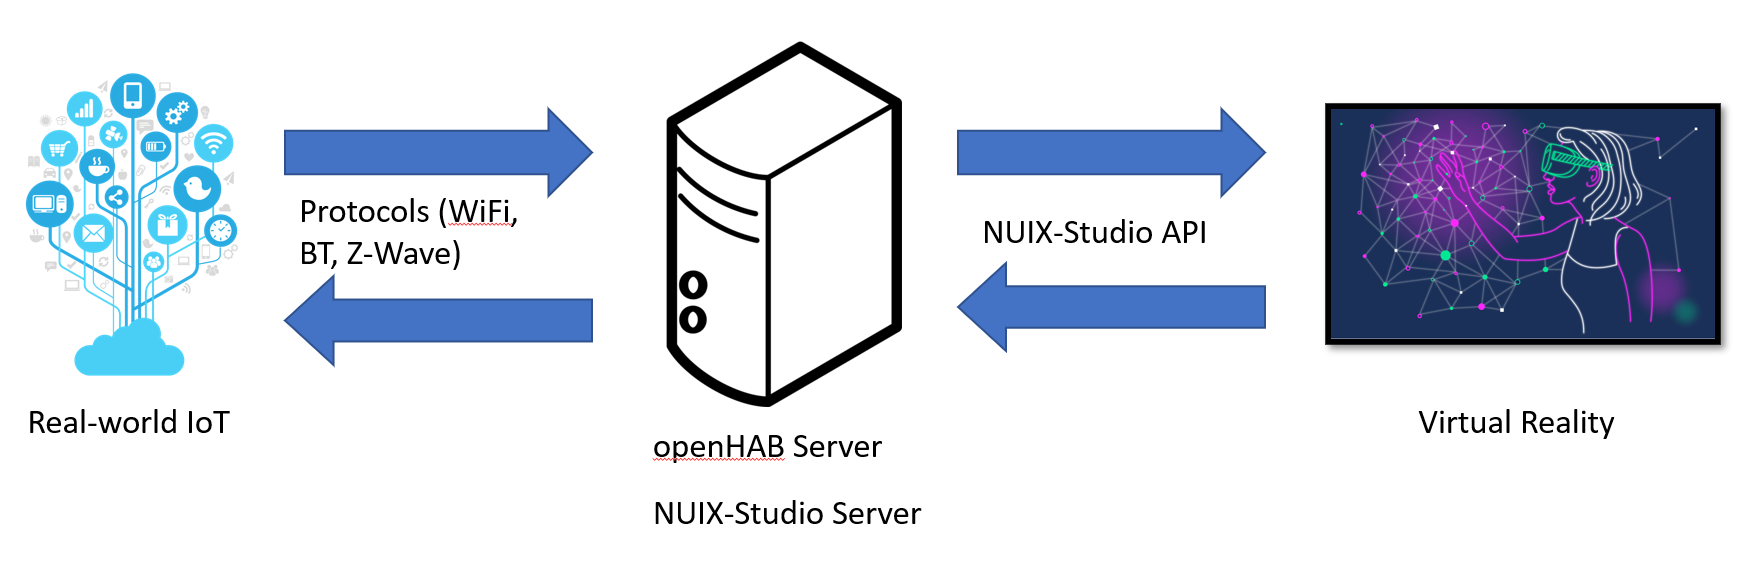
\includegraphics[width=0.9\linewidth]{figures/BasicPlatformStructure.png}
  \caption{Simplified structure of NUIX Studio. Real-world IoT devices HUB is an openHAB server, while NUIX-Studio server is an instance of NUIX-Studio App responsible for the computations.}
  \label{fig:BasicPlatformStructure-figure}
\end{figure}

\section{Server Architecture}
\subsection{OpenHAB Server Structure}

It was decided not to change the openHAB system's structure since it follows the SOA principles that allow implementing support for various types of devices (Figure~\ref{fig:openHABServerStructure-figure}).

\begin{figure}
  \centering
  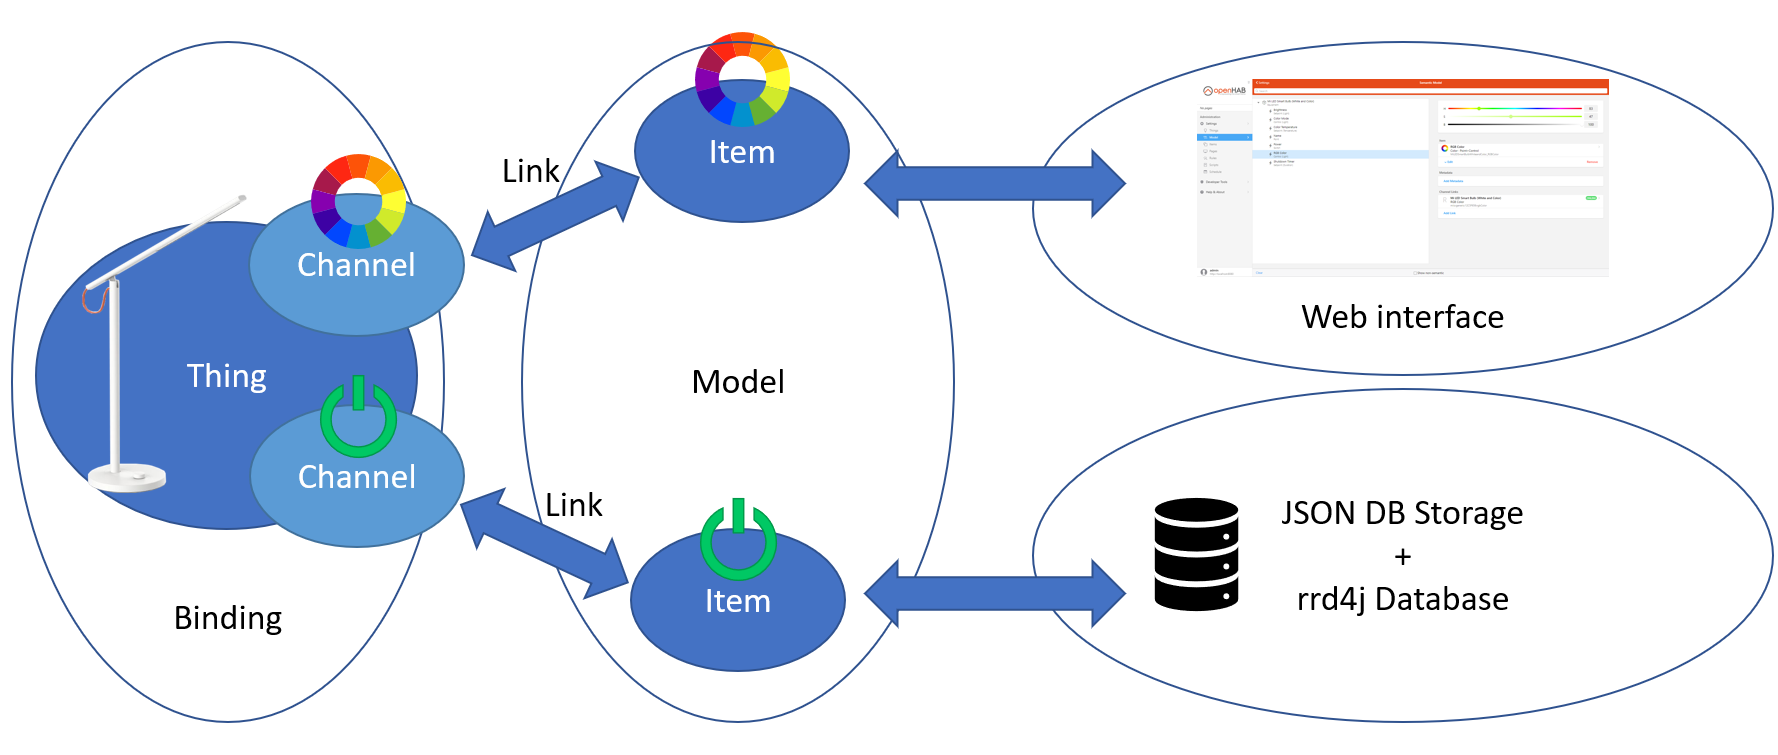
\includegraphics[width=0.9\linewidth]{figures/openHABServerStructure.png}
  \caption{Server structure}
  \label{fig:openHABServerStructure-figure}
\end{figure}

Each IoT device is called a Thing, but a Thing can also be a  service. For example, a smoke sensor and user location are both Things.

Things expose their capabilities through Channels. For example, smart vacuum cleaner channels can be suction strength, water delivery strength, remaining charge level, and cleaning status.

Each channel is associated with one or more Items that are added inside the model. In the example, each of the Items is linked to only one Channel, and each of the channels is linked to only one Item. Items have a State, and they may receive commands. 

Before adding an IoT device to the server, the developer has to install a software adapter first. These add-ons are called bindings, and they provide a way to link Items to physical devices. Most of the protocols for connecting to IoT devices are supported by the corresponding bindings.

For example, after a binding for Xiaomi smart home devices is installed, the smart home devices can be automatically discovered by the server and added as Things. A Xiaomi Lamp is used in the example, for which several Channels are presented (Figure~\ref{fig:XiaomiLampChannels-figure}).

\begin{figure}
  \centering
  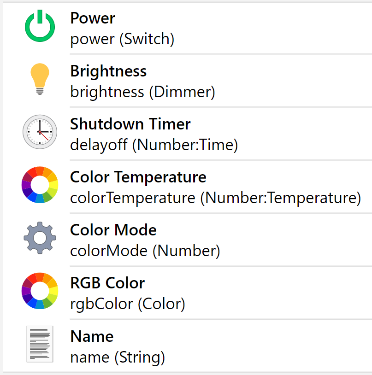
\includegraphics[width=0.6\linewidth]{figures/XiaomiLampChannels.png}
  \caption{Channels list example.}
  \label{fig:XiaomiLampChannels-figure}
\end{figure}

Each of these channels represents one Item (Figure~\ref{fig:XiaomiLampPowerItem-figure}).

\begin{figure}
  \centering
  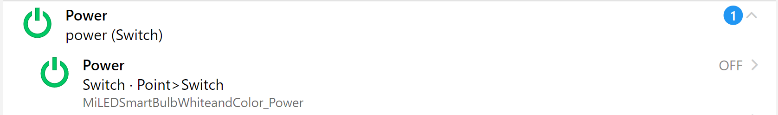
\includegraphics[width=0.9\linewidth]{figures/XiaomiLampPowerItem.png}
  \caption{An Item example.}
  \label{fig:XiaomiLampPowerItem-figure}
\end{figure}

For example, the Power Control is performed through the power channel. In terms of the introduced concepts, the Power Control is an Item named "MiLEDSmartBulbWhiteandColorPower" of type Switch and State "OFF."

As soon as the lamp is turned On, the Power Control switch in Web Interface will also turn ON. And if the switch is changed to the "OFF" state in the Web Interface, the lamp will automatically turn off.

\subsection{Server Extended Structure}

In the previous section, it was not specified how the platform should perform access to the server data. Syncing is performed through REST API (Figure~\ref{fig:ExtendedServerStructure-figure}) , which is explained in detail in Table~\ref{tab:rest-api-table}.

\begin{figure}
  \centering
  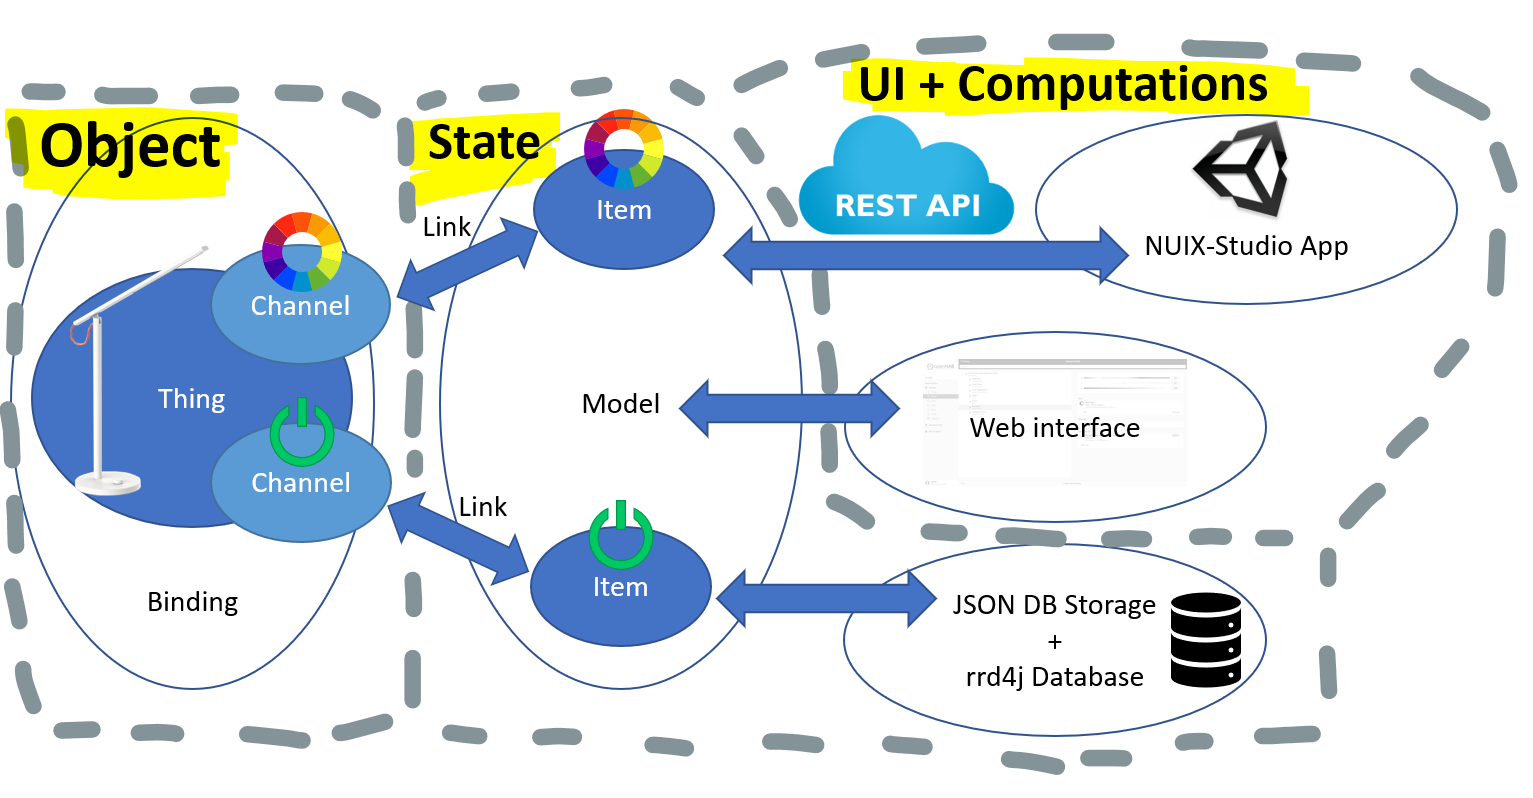
\includegraphics[width=0.9\linewidth]{figures/ExtendedServerStructure.png}
  \caption{Structure of the server showing how the NUIX-Studio App is connected to it.}
  \label{fig:ExtendedServerStructure-figure}
\end{figure}

\begin{table}
  \centering
  \begin{threeparttable}[c]
    \caption{REST API commands used in NUIX-Studio}
    \label{tab:rest-api-table}
    \begin{tabular}{ll}
      \toprule
      REST API CALL    &         DESCRIPTION                 \\
      \midrule
      GET\tnote{a} & Get all available items \\
      POST\tnote{b} & Adds a new item to the registry or updates the existing item    \\
      PUT\tnote{b}        & Sends a command to the item                              \\
      DELETE\tnote{b}        & Removes an item from the registry          \\
      \bottomrule
    \end{tabular}
    \begin{tablenotes}
      \item [a] For link: /items
      \item [b] For link: /items/<itemname>
    \end{tablenotes}
  \end{threeparttable}
\end{table}

In the current implementation of the platform, four different REST API commands are used: GET command for receiving the Items in the registry on system startup, PUT command to create a new Item on the server, POST command for updating the state of the Item, and DELETE command for removing an Item from the server.

States of the Items are received by getting the events from the server: once the event is received, the Item state can be retrieved from the Data Transfer Object's (DTO) payload.

\section{NUIX-Studio App}

As mentioned above, there can be several NUIX-Studio App instances running at the same time. Each of them has access to the Server through REST API. The instances can be of one of the three types:

\begin{enumerate}
    \item Virtual Reality Instance. It runs on Oculus or another VR headset, has remote or local access to the server. Items received from the server are visualized. It is possible to interact with the Items in different ways through touching buttons, moving sliders, performing hand gestures, using voice commands, etc. 
    \item Computations Instance. It runs on a powerful machine and has either remote or local access to the server. Since latency is important for the VR-IoT platform's performance, it is preferable to run this instance on the same machine as the openHAB server. In this case, the REST API calls time will be less than the minimum measurement unit (compared to milliseconds for accessing remote virtual reality instances)\footnote{An experiment to prove this statement is provided in Chapter 4.}. Physics, Big Data analysis, and other performance-based computations are executed in this instance, while user interactions are limited.
    \item Input simulation instance. If the App instance runs on the device with limited support of virtual reality interaction interfaces (for example, a PC), input simulation can be used. Sometimes, it is even easier to run and test the platform on such devices: for example, if using a physical keyboard is required or when there is no access to a VR headset.
\end{enumerate}

Each of the instances has access to the same data on the server, making it possible to work simultaneously in one virtual environment and divide tasks between several NUIX-Studio App instances (Figure~\ref{fig:AppInstances-figure}). One of the instances can be used for computations, while others can be used for interacting with the devices in Virtual reality.

\begin{figure}
  \centering
  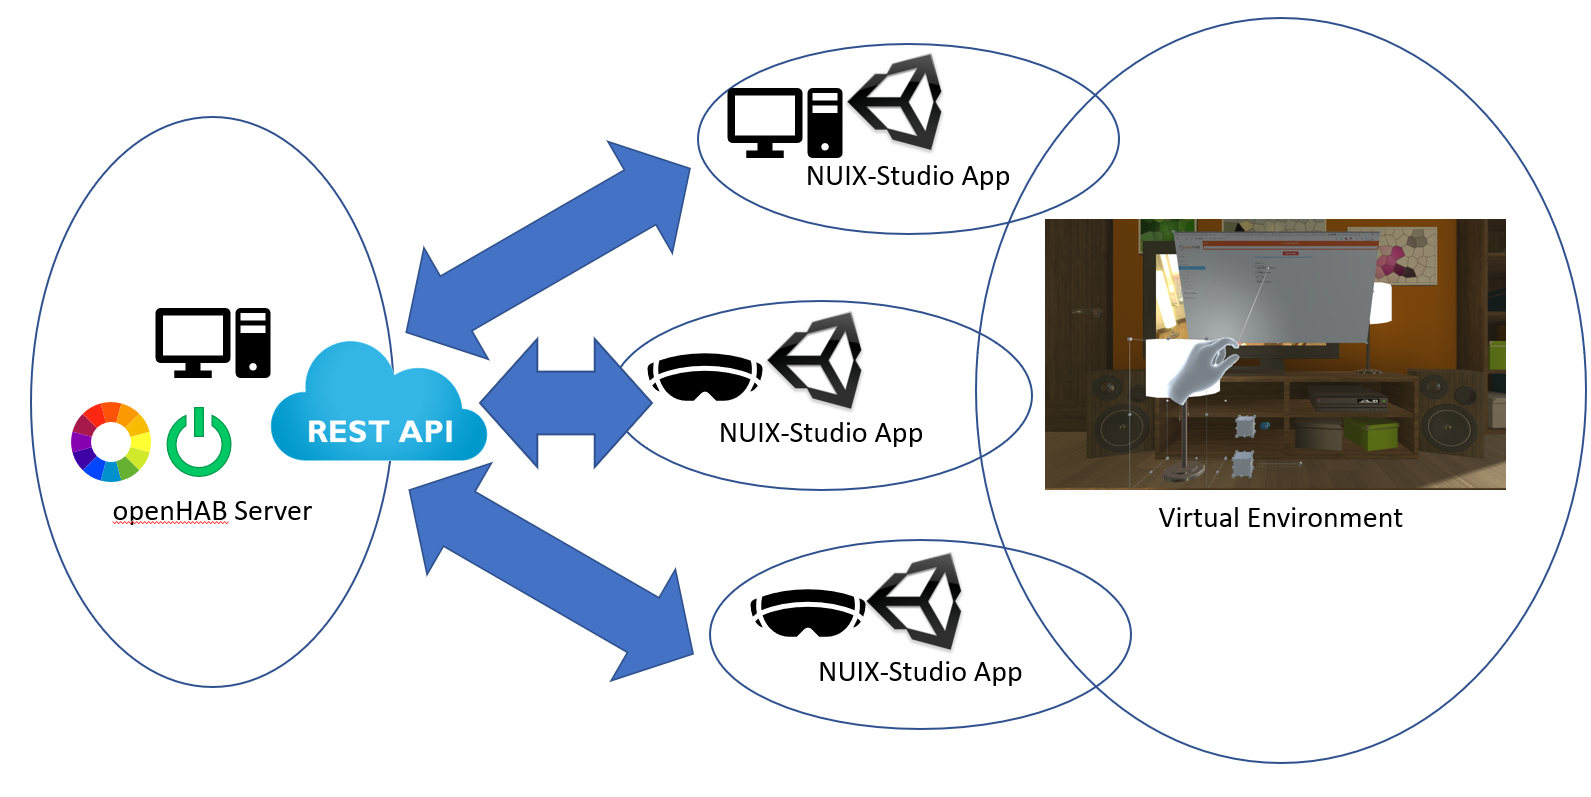
\includegraphics[width=0.9\linewidth]{figures/AppInstances.png}
  \caption{NUIX-Studio App Instances}
  \label{fig:AppInstances-figure}
\end{figure}

\subsection{NUIX-Studio App Architecture}

After the NUIX-Studio App requests access to the system to get the list of items from the registry, a list of Item Data Transfer Objects is received by the App and then added into Semantic Model (Figure~\ref{fig:AppArchitecture-figure}). After the Item state is updated or an Item is added or removed, an event is sent to the EventController instance, and then, based on the event payload, the Item list is updated.  By keeping each Item data on the device equal to the Item data on the server, the Semantic model in NUIX-Studio App remains equivalent to the Semantic model presented on the server. 

\begin{figure}
  \centering
  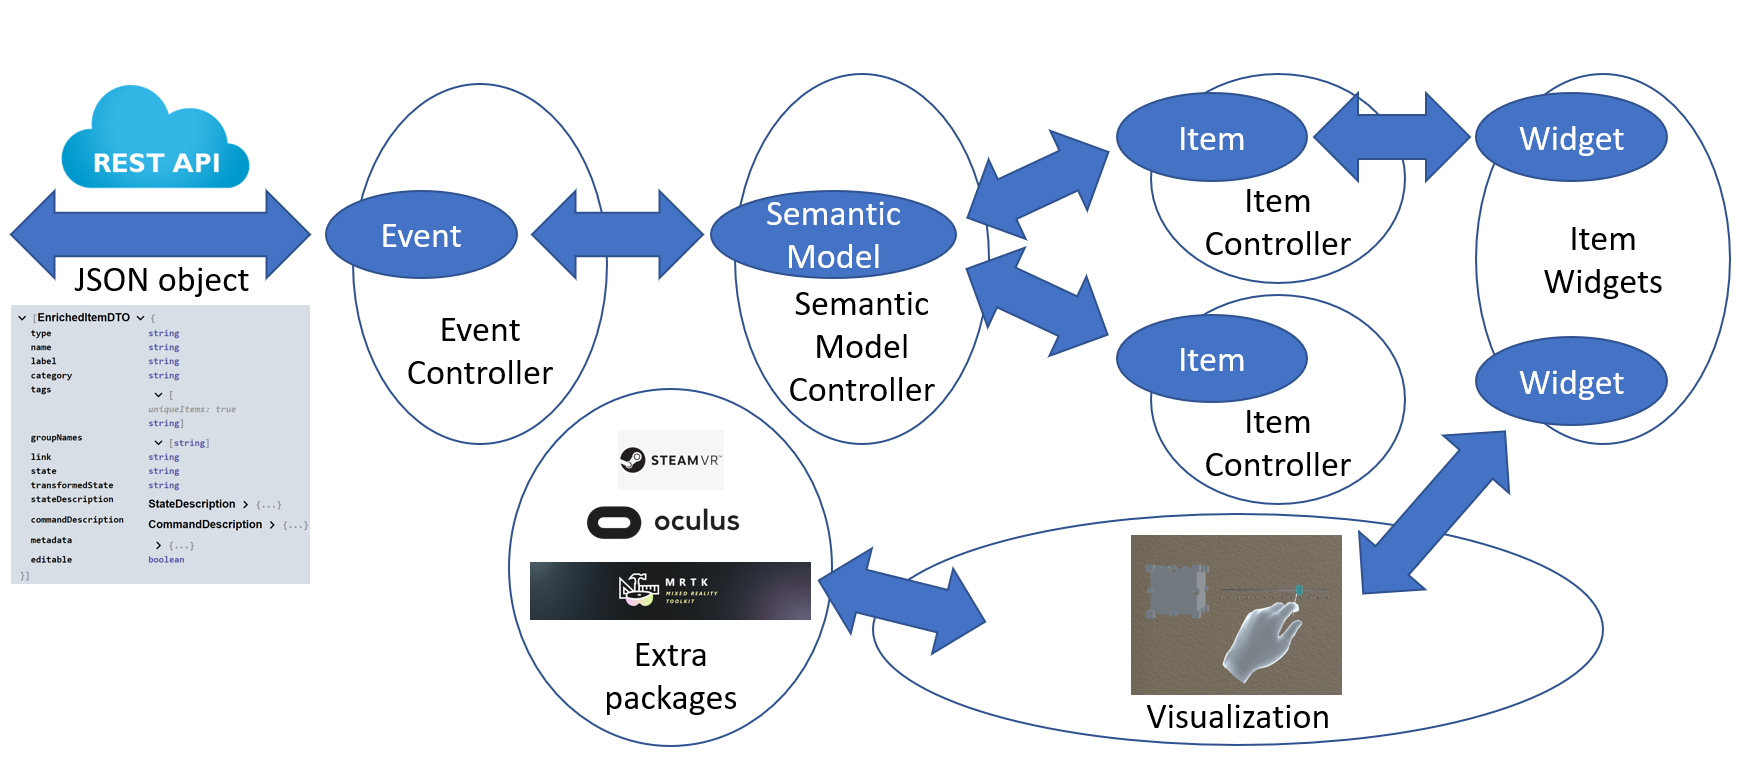
\includegraphics[width=0.9\linewidth]{figures/AppArchitecture.png}
  \caption{NUIX-Studio App Architecture}
  \label{fig:AppArchitecture-figure}
\end{figure}

But only storing the states of the Items in the App does not allow users to interact with the IoT devices. In other words, NUIX-Studio App has to provide an interface to interact with the Items. Since different types of Items require different interaction techniques, a Widget object is created for each item type to solve this issue.
Widget in NUIX-Studio App is a Unity Virtual object, which can visualize the Item state and update it. For example, it can be an interactable pinch slider for a dimmer Item or a virtual screen for an Image item.

By integrating Extra frameworks, NUIX-Studio platform can provide a wider variety of Widgets and a higher number of supported devices. For example, Oculus Integration support provides an API for hands recognition; SteamVR (\cite{SteamVR2021}) support makes it possible to run the NUIX-Studio App on the majority of VR headsets.

\subsection{NUIX-Studio App Semantic Model}

As mentioned above, the Semantic model in the NUIX-Studio App is kept equivalent to the Semantic model stored on the server. The advantages of this approach are listed below:

\begin{enumerate}
    \item Each of the App instances visualizes equivalent data, providing simultaneous and fault-tolerance work;
    \item The Semantic model on the server is time- and memory-effective. Hence, the Semantic model in the App is also time- and memory-effective.
\end{enumerate}

Overall, using the defined approach, the platform follows the Dependency-inversion principle. In this case, both the Semantic model and Item are abstractions.

But when it is required to provide an interface for creating new IoT devices in VR and interaction with them, it is not possible to use items presented on the server only. For example, each Item's virtual position inside the VR environment is a required data, which should be accessible by each of the instances.

The platform's main purpose is to provide an interface to test new IoT devices inside Virtual reality or extend the existing items with extra functionality. But only real-world devices' data is stored on the server. Therefore, the Semantic model should be extended with extra items. 